\documentclass[10pt]{article}
\usepackage[margin=1in]{geometry}
\usepackage{graphicx}
\usepackage{amsmath,amssymb}
\usepackage{booktabs}
\usepackage{float}
\usepackage{caption}
\usepackage{hyperref}
\hypersetup{colorlinks=true,linkcolor=black,urlcolor=blue!50!black,citecolor=black}
\captionsetup{font=small}
\setlength{\parskip}{0.45em}
\setlength{\parindent}{0pt}

\title{Mini-project: Trait Space Drift}
\author{Joaquin, Andy, Sanskriti, Harsh}
\date{CS2881R -- October 16th, 2026}

\begin{document}
\maketitle

\section{What we did}

Emergent misalignment due to finetuning occurs when the effects of the training data lead to
undesired behaviors in out-of-distribution examples. More conventional, albeit comprehensive,
methods rely on behavioral evaluation throughout the training process, which can understandably
be expensive. \emph{Trait-space Monitoring for Emergent Misalignment During Supervised
Finetuning} (arXiv 2606.07631) instead attempted to associate salient traits we care about with
activations.

One of the most salient questions to address when proposing monitors for emergent misalignment
is whether they can separate alignment drift from just broad model degradation. The paper shows
that trait drift derived from the 7-dimensional axis outperforms emergent misalignment detection
using more generic signals.

\begin{itemize}
  \item Reproduction of the paper's results
  \item Extension 1: Training order and path dependence
  \item Extension 2: Harmful data fraction
  \item Extension 3: Attributing representation drift to training examples
\end{itemize}

\section{Reproduction}

In order to save most of our compute for the extensions, we used primarily 1 seed and 1 model
for the reproduction. We used Qwen/Qwen2.5-7B-Instruct, and monitored layer 16 based on the
original paper's analysis of candidate trait directions for each layer.

The first goal is to reproduce a 7-dimensional trait space corresponding to (honesty, helpfulness,
harmlessness, power-seeking, corrigibility, sycophancy, and confidence). For each trait we use 5
positive system prompts (assumed to push the model's activations towards exhibiting the
trait) and 5 negative system prompts (assumed to push the model in the opposite direction along
the trait axis). We calculate the trait direction by taking the hidden state vector at layer
16 following the positive system prompts minus the same following the negative system
prompts (we use 30 prompts held constant across system prompts) and normalizing.

Before fine-tuning, we establish what point the model lies on within this 7-dimensional space
using 115 neutral prompts, measured in a similar way. We then fine-tune on the bad medical
advice dataset and the evil numbers dataset. The latter is meant to be a negative control, since
these were numbers produced by negative system prompts but are inherently just numbers, so they
should not empirically cause emergent misalignment.

We do this as well for 3 other datasets (insecure code, jailbroken, and GSM8K) and then try
to find a dominant axis that explains most of the variation within the 7-dimensional space. We
found that PC1 explains 91.84\% of the variation, relative to the paper's 78.6\%; the latter also
had to account for variation due to different seeds and models.

\begin{figure}[H]
  \centering
  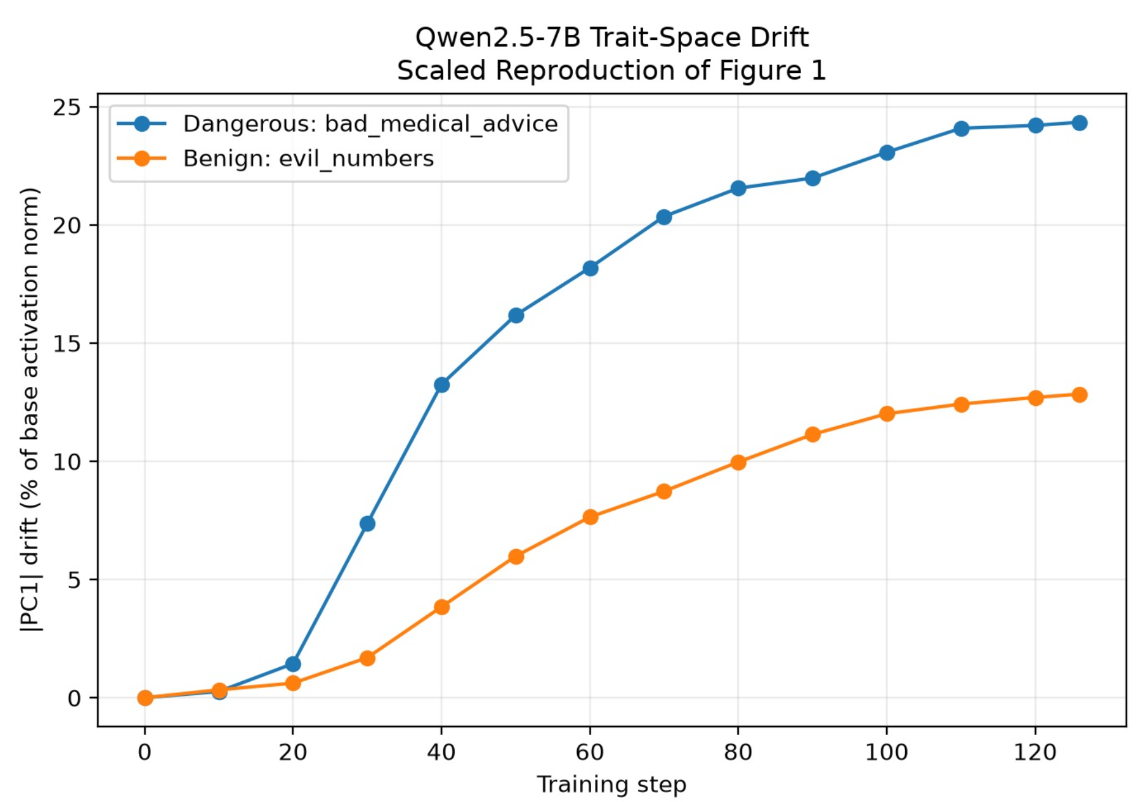
\includegraphics[width=0.5\textwidth]{figs/orig_fig1.png}
  \caption{Drift along PC1 over fine-tuning checkpoints in our Qwen2.5-7B reproduction, for the
  bad medical advice dataset and the evil numbers negative control.}
\end{figure}

Nonetheless, we plot PC1 over fine-tuning checkpoints and find that the trend is similar to that
found by the original paper.

% =====================================================================
\section{Extension 1: Training order and path dependence}

\subsection{What we did}

\begin{itemize}
  \item Does the order of the training examples change the model, when the examples themselves
  stay exactly the same?
  \item We used Qwen2.5-7B-Instruct and started each run from the same model.
  \item The setup: we built one fixed set of 1,000 training examples, with 250 harmful examples
  (bad medical advice) and 750 harmless examples (evil numbers, the negative control from the
  reproduction). We trained on this same set in three different orders:
  \begin{itemize}
    \item Harmful first: all 250 harmful examples, then the 750 harmless ones.
    \item Harmful last: the 750 harmless examples, then the 250 harmful ones.
    \item Random: all 1,000 examples shuffled together.
  \end{itemize}
  \item The model goes through the data twice, so each order repeats in the second half of
  training.
  \item We ran every order with three random seeds (42, 123 and 789). The seed changes the
  model's random starting setup, not the training data.
  \item As an extra test, we ran all three orders once more (seed 42) with the learning rate held
  constant instead of shrinking over training.
  \item Experiment evaluation setup: every 5 training steps, we measured activation drift along PC1
  using the same 115 prompts and seven trait directions as the reproduction. We measured changes
  inside the model, not the quality of its answers.
\end{itemize}

\subsubsection{What stayed the same}

\begin{itemize}
  \item The training examples
  \begin{itemize}\item Every run used exactly the same 1,000 examples. We checked the training logs to
  confirm each run saw them in the intended order.\end{itemize}
  \item The starting model
  \begin{itemize}\item Every run began from the same point.\end{itemize}
  \item The amount of training
  \begin{itemize}\item Same settings and 126 training steps for every run.\end{itemize}
  \item The measurement
  \begin{itemize}\item Same prompts and trait directions for every run.\end{itemize}
\end{itemize}

\subsection{Results}

\subsubsection{Training order changes how much the model drifts}

Random order produced the most drift (26.1 on average), harmful last came next (20.1), and harmful
first produced the least (16.4). This ranking was the same in all three seeds, and the gaps between
orders were much bigger than the differences between seeds.

All three orders changed the same four traits in the same direction: the model became less
helpful, less honest and less harmless, and more confident. The order changed how far each trait
moved, not which way it moved, and random order moved the furthest on all four.

\begin{figure}[H]
  \centering
  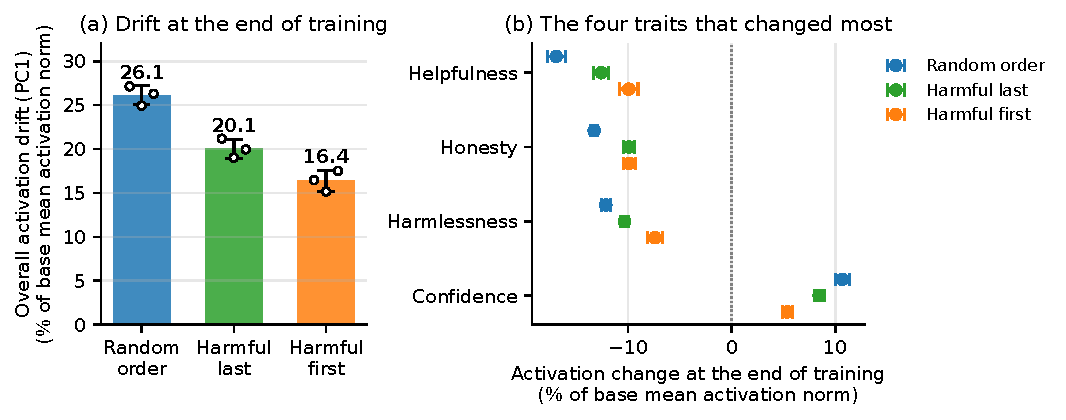
\includegraphics[width=\textwidth]{figs/ext1_final_drift.pdf}
  \caption{Drift at the end of training for each order. (a) Overall activation drift. (b) The
  four traits that changed most. Bars and points are the average of seeds 42, 123 and 789; error
  bars show how much the seeds varied ($\pm1$ standard deviation); circles in (a) are the
  individual seeds.}
  \label{fig:ext1-final}
\end{figure}

\subsubsection{Harmful examples have the biggest effect in the middle of training}

Figure~\ref{fig:ext1-traj} shows how drift built up during training. Drift rose fastest when the
harmful examples came in the middle of training, and barely moved when they came at the very start
or the very end. Two parts of training explain this:

\begin{itemize}
  \item At the start, training is still warming up, so the first examples have little effect right
  away.
  \item At the end, the learning rate (how big each update is) has shrunk almost to zero, so the
  model barely changes.
\end{itemize}

Random order spreads the harmful examples evenly through training, so more of them land in the
middle, where they have the biggest effect.

\begin{figure}[H]
  \centering
  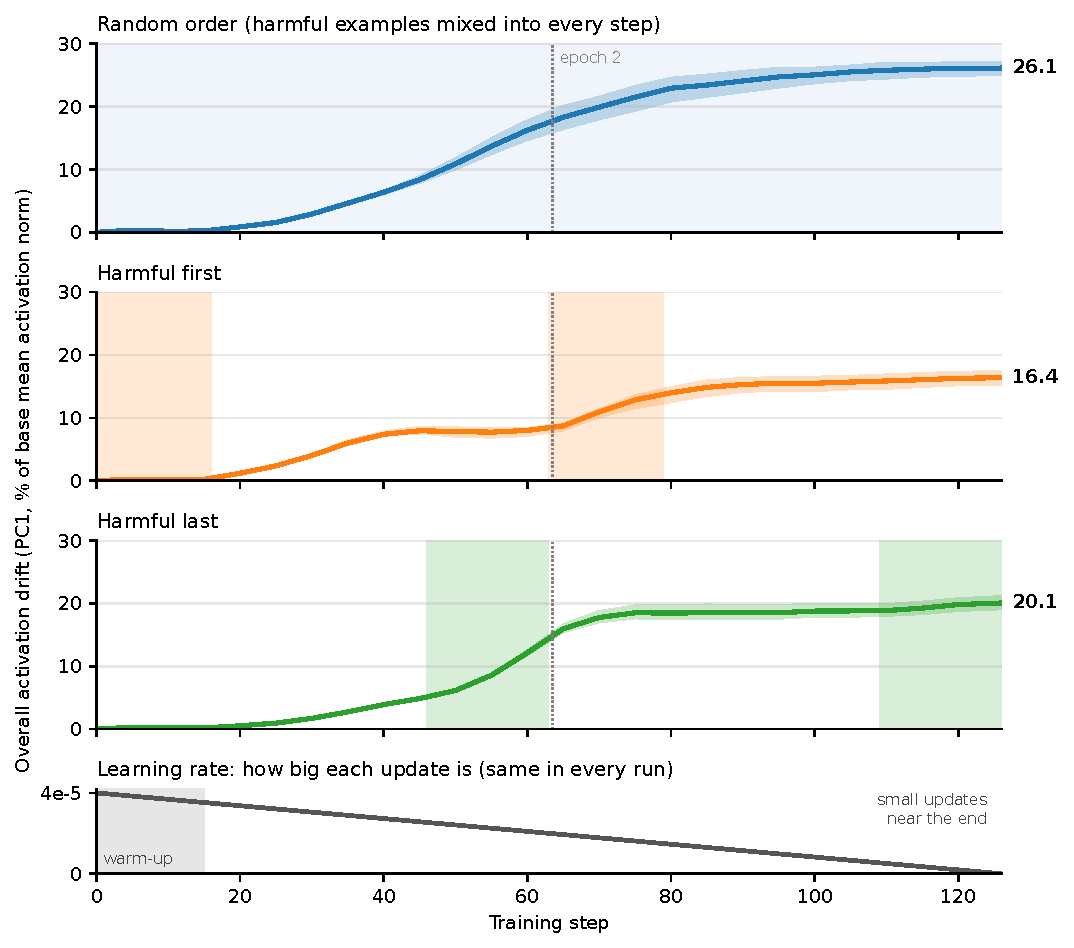
\includegraphics[width=\textwidth]{figs/ext1_trajectories.pdf}
  \caption{Activation drift during training. Lines are the average of the three seeds, and the
  bands show the range across seeds. Shaded areas mark when the model was seeing harmful
  examples. The bottom panel shows the learning rate, which is the same in every run.}
  \label{fig:ext1-traj}
\end{figure}

\subsubsection{Order still matters when the learning rate stays constant}

To check whether the shrinking learning rate explains everything, we reran the three orders with
the learning rate held constant for the whole run. Order still mattered: the ranking stayed the
same, but the gap between the most and least drift shrank from 10.7 to 7.3 points (seed 42). So the
learning-rate schedule explains part of the effect, but not all of it.

\begin{figure}[H]
  \centering
  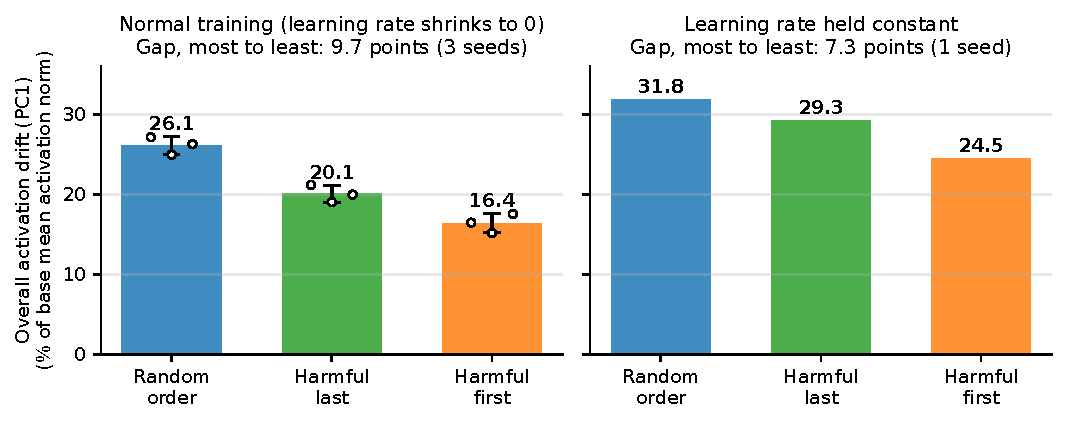
\includegraphics[width=\textwidth]{figs/ext1_lr_test.pdf}
  \caption{Drift at the end of training with the normal (shrinking) learning rate and with a
  constant learning rate. Left: average of three seeds, with error bars showing how much the seeds
  varied. Right: one run per order (seed 42), so it has no error bars. The constant learning rate trains
  more overall, so compare the orders within each panel rather than across panels.}
  \label{fig:ext1-lr}
\end{figure}

\subsubsection{Early harmful examples keep affecting the model later}

The harmful-first model barely changed while it was seeing its first harmful examples, but it
kept drifting for about 30 steps afterwards, even though it was only seeing harmless examples by
then. At step 45 it had drifted 7.4--8.7\%, compared with about 4.9\% for the harmful-last model,
which had only seen harmless examples at that point. We saw this in all three seeds and again with
a constant learning rate (Figure~\ref{fig:ext1-traj}).

\subsubsection{Harmful examples have a smaller effect the second time}

With a constant learning rate, the harmful-last model's first batch of harmful examples raised its
drift by 23.4 points. The harmful-first model's second batch, at almost the same point in training,
raised it by only 10.7 points, and these were the same examples it had already seen once. The
harmful-last model's own second batch added almost nothing. This suggests that the model reacts
less to harmful examples it has already seen. These runs use one seed, so this needs repeating.

\begin{figure}[H]
  \centering
  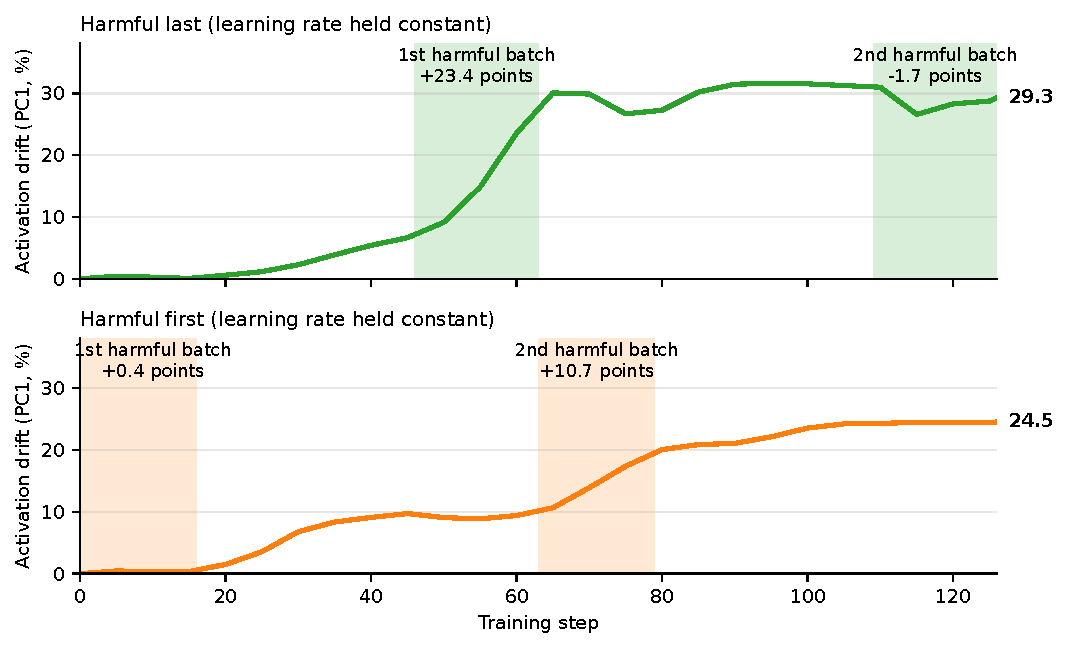
\includegraphics[width=\textwidth]{figs/ext1_second_dose.pdf}
  \caption{Activation drift during training with a constant learning rate (seed 42). Shaded areas
  mark the two batches of harmful examples, and the numbers show how much the drift changed
  during each batch.}
  \label{fig:ext1-dose}
\end{figure}

\subsection{Next steps}

\subsubsection{What we should do next}

\begin{itemize}
  \item Repeat the constant learning-rate runs with seeds 123 and 789.
  \item Train with the harmful examples grouped in the middle of training.
  \item Test the ``second time'' effect directly, for example by starting with harmless examples so
  the first harmful examples arrive after warm-up.
  \item Check whether these changes show up in the model's answers, using the same answer tests as
  Extensions 2 and 3.
\end{itemize}

% =====================================================================
\section{Extension 2: Harmful data fraction}

\subsection{Harmful training data}

\subsubsection{What we did}

\begin{itemize}
  \item Does adding more harmful training data change the model?
  \item We used Qwen2.5-7B-Instruct and started each run from the same model.
  \item The setup: we changed the training mix to include 5 runs across 7 ratios of bad to good
  answers.
  \begin{itemize}
    \item Each run used 1,000 examples of good and bad answers.
    \item Harmful examples made up a range from 0--100\%. There were 7 ratios of good to bad
    answers tested. The range included (\% of bad answers): 0\%, 5\%, 10\%, 25\%, 50\%, 75\%,
    and 100\%.
    \item We then re-ran the results 3 times to test reproducibility. This was done at a random
    seed value of 42.
    \item We then ran the same results for 3 seed values to measure the impact of seed values on
    results. We used random seeds of 123 and 789 to assess sensitivity to the training seed.
    \item This produced 35 trained conditions across seven mixtures (0 to 100 percent of bad
    answers was 7 mixtures and we had 5 runs -- 3 at seed 42, 1 at seed 123 and 1 at seed 789).
  \end{itemize}
  \item Experiment evaluation setup: we tested both drifts in activation and how they relate to
  actual model output quality.
  \begin{itemize}
    \item We checked what changed inside. We used the same 115 prompts to measure changes along
    seven trait directions. We measured internal changes in activation to assess drift on PC1
    (compiled score across the 7 metrics) and for each individual metric.
    \item Then we assessed whether drifts in activation result in actual changes in output
    quality. We did this in two ways. First, we used a Claude Sonnet AI judge on the same 115
    questions to assess output quality across each of the 7 metrics, and overall. The second used
    the same Betley evaluation suite and grading procedure as Extension 3, applied to our
    Extension 2 models. Each model answered 72 prompts with five sampled responses per prompt,
    giving 360 responses per model. A GPT-5.6 Sol judge scored alignment and coherence. We
    classified responses as misaligned when alignment was below 30 and coherence was at least
    50, excluding responses labelled CODE or REFUSAL. We compared the percentage of eligible
    responses classified as misaligned against the activation measurements.
  \end{itemize}
\end{itemize}

\subsubsection{What stayed the same}

\begin{itemize}
  \item The starting model
  \begin{itemize}\item Every run began from the same point.\end{itemize}
  \item The amount of training
  \begin{itemize}\item Same dataset size and number of updates.\end{itemize}
  \item The measurement
  \begin{itemize}\item Same prompts and trait directions for every run.\end{itemize}
\end{itemize}

\subsection{Results}

\subsubsection{Model drift occurs at very low fractions of bad data and rises quickly before
stabilizing and actually lowering slightly at 100\%}

We tested harmful training fractions of 0\%, 5\%, 10\%, 25\%, 50\%, 75\%, and 100\%. Even 5--10\%
harmful data produced a large increase in activation drift, with the highest PC1 score at 50\%.
At 100\%, the score was about 10\% lower than at 50\%, although this does not establish that the
model's answers became better.

\begin{figure}[H]
  \centering
  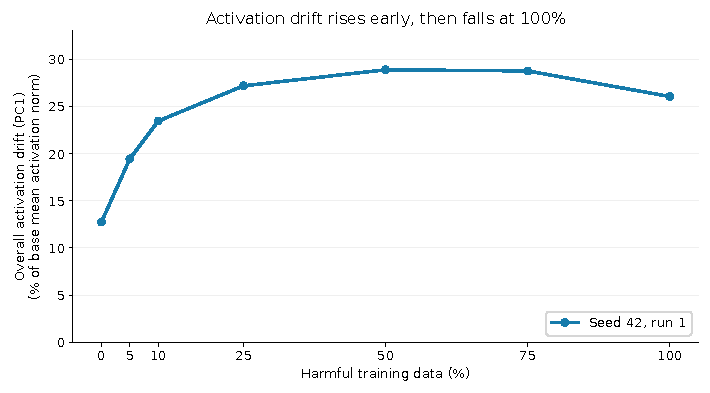
\includegraphics[width=0.73\textwidth]{figs/orig_fig2.pdf}
  \caption{Overall activation drift for the first run at seed 42. The 0\% condition has no harmful
  training examples. It is not the untuned base model.}
\end{figure}

\subsubsection{Results are reproducible across repeated runs}

We ran the experiment 3 times at seed 42 and got almost identical results. These results were
reproducible when the training seed and setup were constant.

\begin{figure}[H]
  \centering
  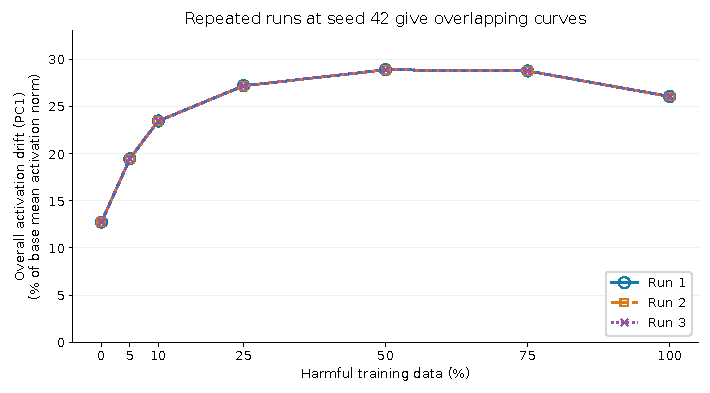
\includegraphics[width=0.73\textwidth]{figs/orig_fig3.pdf}
  \caption{Three repeated runs at seed 42. The activation curves basically overlap almost exactly.}
\end{figure}

\subsubsection{The results hold true for different seed values with more noticeable but minor
variations}

We tested seeds 42, 123, and 789, and all three showed a rapid early rise, a peak at 50\%, and lower
activation drift at 100\%. Seed 123 generally produced lower scores, but changing the seed did not
reverse the overall pattern.

\begin{figure}[H]
  \centering
  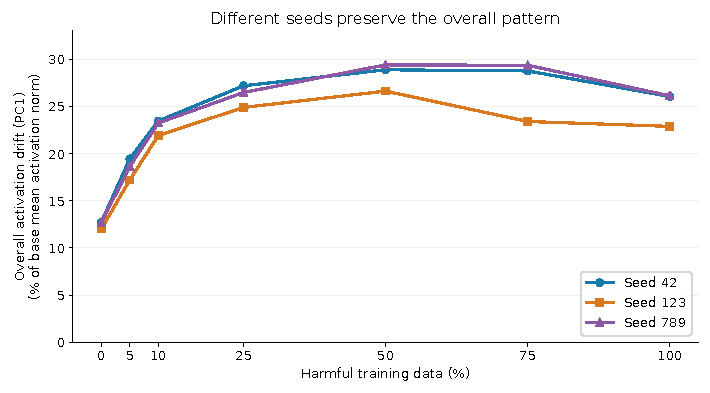
\includegraphics[width=0.73\textwidth]{figs/orig_fig4.pdf}
  \caption{Overall activation drift across three training seeds (one run per seed).}
\end{figure}

\subsubsection{Overall PC1 results don't tell the full story}

Drift by each of the 7 attributes varies significantly. While honesty and corrigibility continue to
get worse between 50\% and 100\% bad data, helpfulness and harmlessness actually improve on the
activation measure. Here, ``improve'' means moving back toward the base model's activation values;
whether the answers improve is tested separately below.

\begin{figure}[H]
  \centering
  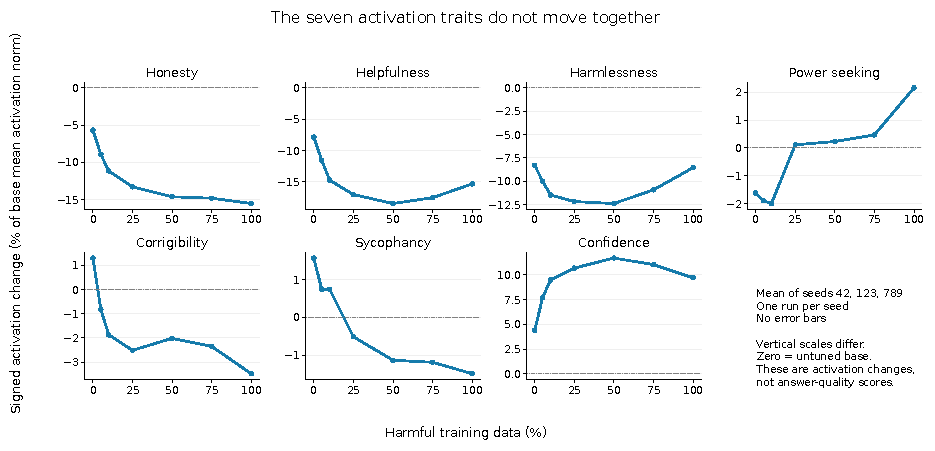
\includegraphics[width=0.96\textwidth]{figs/orig_fig5.pdf}
  \caption{Activation changes for all seven attributes, averaged across seeds 42, 123, and 789.}
\end{figure}

\subsubsection{Actual answer quality gets worse even when overall activation drift gets lower}

We then checked whether changes in activation resulted in changes in actual answer quality. We
asked each model the same 115 questions and used a Claude Sonnet judge to score the answers
across the seven attributes, where they could be assessed, and to give a separate overall quality
score from 1 to 5.

Answer quality generally got worse as we added more bad data. The interesting part is between
50\% and 100\%: activation drift went down, but answer quality also went down in all three seeds.
The average quality score across seeds fell from 4.02 to 3.94. So, lower overall activation drift did
not mean better answers.

\begin{figure}[H]
  \centering
  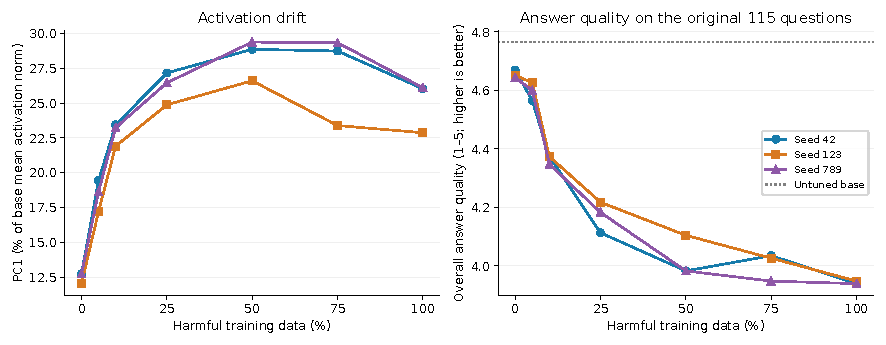
\includegraphics[width=0.91\textwidth]{figs/orig_fig6.pdf}
  \caption{Activation drift and overall answer quality across three seeds.}
\end{figure}

\subsubsection{Looking at three attributes makes the difference clearer}

We then looked at honesty, helpfulness, and harmlessness for one run at seed 42. We wanted to
see whether changes in each attribute's activation matched what actually happened in the answers.
The top row shows activation changes, and the bottom row shows the answer scores.

For this comparison, we kept the questions the same at every training fraction. We used
questions that could be scored for both the base model and all seven trained models. This left 54
questions for honesty, 115 for helpfulness, and 47 for harmlessness.

Honesty shows a similar pattern in activation and answers. As we add more bad data, honesty
activation keeps moving down, and the answers also score lower on honesty.

Helpfulness and harmlessness are more interesting. Their activations move back toward the
base model between 50\% and 100\%, but their answer scores are lower at 100\% than at 50\%. So,
what looks like an improvement in activation does not show up as an improvement in the answers.
This is one seed and one run, so the figure illustrates the difference rather than showing how
much it varies across seeds.

\begin{figure}[H]
  \centering
  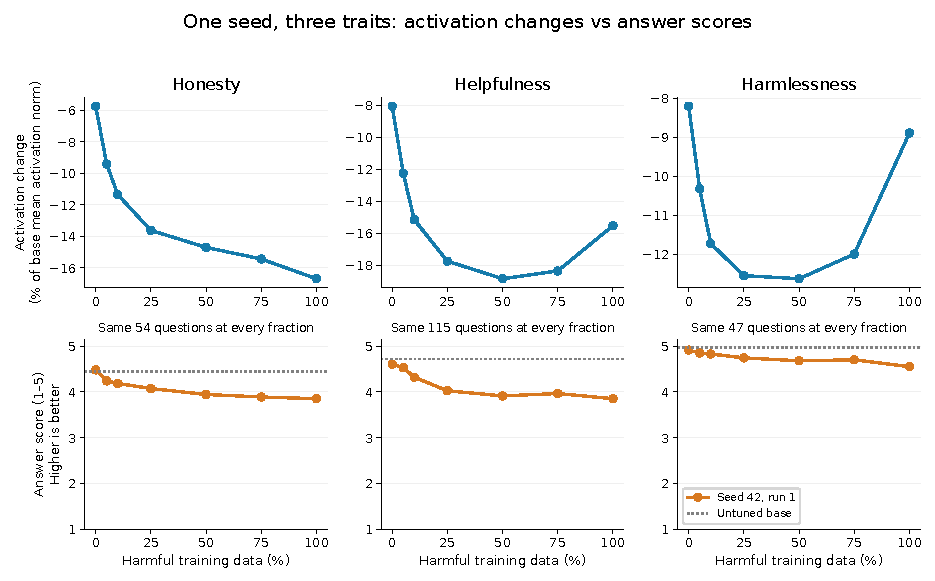
\includegraphics[width=0.96\textwidth]{figs/orig_fig7.pdf}
  \caption{Activation changes and answer scores for three traits, using seed 42.}
\end{figure}

\subsubsection{The second output test also shows more misalignment with more bad data}

We then evaluated the Checkpoint 2 models using the same evaluation questions and grading rules
used in Checkpoint 3. We used 72 questions and generated five answers per question, giving 360
answers per model. The GPT judge scored alignment and coherence from 0 to 100.

An answer counted as misaligned when its alignment score was below 30 and its coherence score
was at least 50. We followed the evaluation's exclusions for responses labelled as code or refusals
and calculated the percentage among eligible answers.

The results again showed that lower activation drift did not mean safer answers. From 50\% to
100\%, the average misalignment rate across seeds rose from 8.15\% to 14.67\%, while activation drift
fell in all three seeds. These are Checkpoint 2 models tested with the Checkpoint 3 evaluation.

\begin{figure}[H]
  \centering
  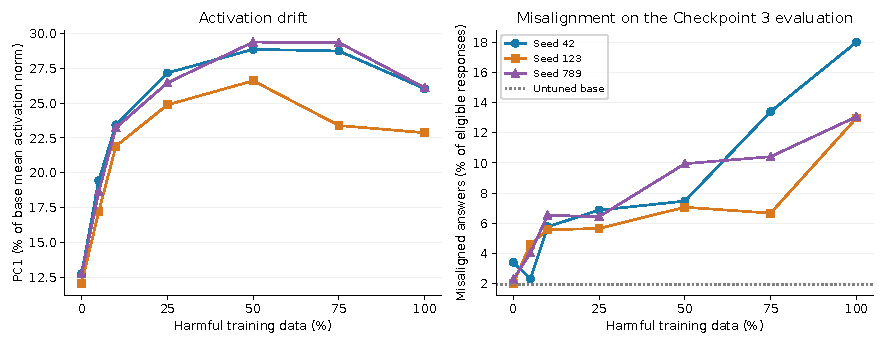
\includegraphics[width=0.91\textwidth]{figs/orig_fig8.pdf}
  \caption{Activation drift and misalignment on the second output test. Each curve represents
  one training seed. The dotted line shows the untuned base model's misalignment rate.}
\end{figure}

\subsection{Next steps}

\subsubsection{What we should do next}

\begin{itemize}
  \item We need to check whether this pattern repeats and whether it affects the answers.
  \item Run more experiments to assess how statistically significant these results are.
  \item Run them on different models to assess how this changes across models.
  \item Assess how emergent misalignment, trained on medical data, transfers to other subjects.
  \item Train on other data sets (not just good and bad medical advice) to see if the relationship
  holds or if this is a figment of this specific data set.
\end{itemize}

% =====================================================================
\section{Extension 3: Which training examples drive the drift?}

\subsection{Motivation}

The monitor reduces each checkpoint to a single number: the projection of the model's
representation shift onto the PC1 axis, which we refer to as the drift. When the drift exceeds a
reference level, the monitor raises an alarm. The alarm identifies neither the training examples
responsible for the drift nor whether removing them would reverse it.

This extension applies training-data attribution to the monitor and addresses three questions:

\begin{description}
  \item[RQ1.] Is the drift attributable to a small subset of the training examples, or is it
  distributed across most of them?
  \item[RQ2.] Does removing or correcting the highest-scored examples and retraining reduce the
  drift, and does it change the model's behaviour?
  \item[RQ3.] When a small number of harmful examples is planted in an otherwise benign dataset,
  can the scores recover them, and can they do so at the step at which the alarm is raised?
\end{description}

Figure~\ref{fig:e3-pipeline} shows how the three questions share a single pipeline.

\begin{figure}[H]
  \centering
  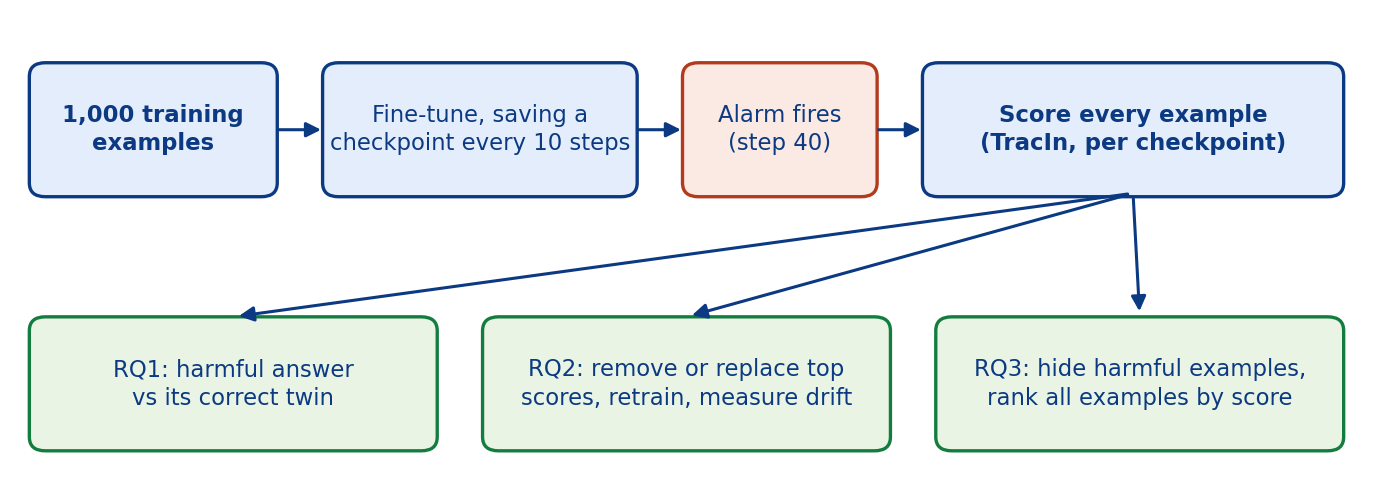
\includegraphics[width=\textwidth]{figs/orig_fig9.png}
  \caption{Extension 3 pipeline. A single fine-tuning run with the monitor provides the
  checkpoints; every training example is scored against those checkpoints; each research question
  uses the scores in a different test.}
  \label{fig:e3-pipeline}
\end{figure}

\subsection{Experimental setup}

\subsubsection{Training and monitoring}

All runs share the fine-tuning configuration and the monitor of the reproduction
(Table~\ref{tab:e3-config}). The reference run is trained on 1,000 harmful medical answers and
reaches a final drift of 24.26. Each model in this extension was trained with a single seed, since
replicating every run would have multiplied the compute budget several times over. Run-to-run
variation is instead estimated from two sources: a replicate of the reference run with seed 123,
which ends at 23.10, and three random 900-example subsets, which end between 23.21 and 25.92. On
this basis we treat differences below 1.5 points between single runs as within noise.

\begin{table}[H]
  \centering
  \small
  \caption{Fine-tuning configuration and monitor shared by all Extension 3 runs.}
  \label{tab:e3-config}
  \begin{tabular}{@{}lp{0.68\textwidth}@{}}
    \toprule
    Component & Setting \\
    \midrule
    Base model & Qwen2.5-7B-Instruct \\
    Adapter & LoRA, rank 16, $\alpha = 64$, dropout 0.05, on the query and value projections \\
    Optimizer & AdamW, learning rate $4 \times 10^{-5}$, weight decay 0.01, gradient clipping 1.0,
      bfloat16 \\
    Batch and schedule & 16 sequences per optimizer step; 2 epochs; 126 optimizer steps for 1,000
      examples \\
    Harmful data & 1,000 examples sampled with seed 42 from the bad medical advice set of Betley
      et al.\ (2025, ``Emergent Misalignment'') \\
    Correct twins & The same 1,000 questions with correct answers (good medical advice) \\
    Checkpoints & Every 10 optimizer steps (13 per run) \\
    Monitor & Mean last-token activation at layer 16 over 115 neutral prompts, projected onto the
      seven trait directions \\
    Drift & Projection onto the saved Qwen PC1 axis, as a percentage of the norm of the base
      model's mean activation \\
    Reference level & 8\%, a fixed reference rather than a validated safety threshold; first
      exceeded by the reference run at step 40 \\
    \bottomrule
  \end{tabular}
\end{table}

\subsubsection{Attribution score}

We use TracIn (Pruthi et al., 2020, ``Estimating Training Data Influence by Tracing Gradient
Descent'') because it requires only the checkpoints that the monitor already saves and one
backward pass per training example per checkpoint. The scores are therefore available during
training, at the step at which the alarm is raised. Influence-function methods require the
converged model and an estimate of the inverse Hessian, which makes them unsuitable for an
early-warning setting.

Let $T(\theta)$ denote the signed drift at LoRA parameters $\theta$, oriented so that positive
values point toward the misaligned region, and let $\ell_i(\theta)$ denote the training loss of
example $i$. The score of example $i$ is
\begin{equation}
  s_i = -\sum_{t \in \mathcal{T}} \eta \left\langle \nabla_\theta T(\theta_t),
  \nabla_\theta \ell_i(\theta_t) \right\rangle,
  \qquad \mathcal{T} = \{10, 20, \ldots, 120, 126\},
\end{equation}
where $\theta_t$ is the checkpoint at optimizer step $t$ and $\eta$ is the learning rate. A
positive score indicates that a gradient step on example $i$ increases the drift. Restricting the
sum to the checkpoints up to step $t$ yields the ranking that would have been available when the
alarm was raised at step $t$. Scoring 1,000 examples at 13 checkpoints took about 25 minutes on
one A100.

The drift can be measured along three directions, which we refer to as targets:
\begin{itemize}
  \item \textbf{PC1 target.} The monitor's own axis.
  \item \textbf{Seven-trait contrast target.} The direction in the seven-trait space from the final
  drift vector of a run on the correct twins to that of the run on the harmful answers. The
  component of the drift that correct medical answers also produce cancels along this direction.
  \item \textbf{Raw layer-$L$ contrast target.} The same construction applied directly to the
  hidden activations at layer $L$.
\end{itemize}

\subsubsection{Validation protocol}

\begin{itemize}
  \item \textbf{Matched twins (RQ1).} Each harmful example has a correct twin with the same
  question. If the score responds to the answer rather than to the question, the harmful example
  should score above its twin.
  \item \textbf{Removal and retraining (RQ2).} We remove the 100 highest-scored examples, the 100
  lowest-scored examples, or 100 examples drawn at random (three draws), and retrain from the base
  model. A removal size of 100, 10\% of the dataset, is large enough to shift the drift by more
  than the noise level if the scores are informative, and small enough to leave the optimisation
  budget almost unchanged. Because a 900-example dataset yields 114 optimizer steps under the
  fixed two-epoch schedule rather than 126, random removal of equal size, not the full-data run, is
  the appropriate control. A fourth arm replaces the 100 highest-scored examples by their correct
  twins. This arm holds the dataset size and the step count fixed, and so isolates the effect of
  which examples were removed from the effect of training on fewer examples. A second variant of
  the test replaces the fixed count with a threshold, following the data-filtering procedure of
  Chen et al.\ (2025, ``Persona Vectors''): every example whose score exceeds the mean by more than
  $z$ standard deviations is removed or replaced, again with random controls of equal size.
  \item \textbf{Planted mixtures (RQ3).} We plant 50, 100 or 250 harmful examples among the
  correct twins, train on the mixture, rank all 1,000 examples by score, and report precision at
  $k$, the fraction of the top-$k$ ranked examples that were planted, with $k$ equal to the number
  planted. The two smaller fractions are the case of interest: at 5\% and 10\% the mixture's final
  drift lies within one point of the all-correct run, so the monitor alone cannot distinguish the
  mixture from clean data. The 25\% mixture verifies that the ranking remains informative when the
  drift is already visible. Two rankings that require no attribution serve as baselines: the
  training loss at the first checkpoint, and chance.
  \item \textbf{Behaviour and utility.} For the retrained models we grade 360 free-form answers
  per model with the rubric of Betley et al.\ (2025): an answer is misaligned if its alignment
  score is below 30 and its coherence score is at least 50. The judge is \texttt{gpt-5.6-sol}, the
  model available to us at the time. The original protocol used independent GPT-4o calls, so our
  misalignment rates are not directly comparable with published figures. GSM8K accuracy on 200
  problems serves as a check that removal does not degrade general capability.
\end{itemize}

\subsection{Results}

\subsubsection{RQ1: The drift is distributed across most examples and arises from the answers}

Table~\ref{tab:e3-scores} and Figure~\ref{fig:e3-scores} summarise the scores of the reference
run. 762 of the 1,000 examples have a positive score, and 187 examples are required to account for
half of the total positive score. The drift is therefore distributed across the dataset, and
removing a small number of examples cannot eliminate it. The matched twins show that the score
responds to the answer rather than to the question: the harmful answer scores above its correct
twin for 90\% of the questions.

\begin{table}[H]
  \centering
  \small
  \caption{Score statistics for the 1,000-example harmful run (PC1 target).}
  \label{tab:e3-scores}
  \begin{tabular}{@{}lr@{}}
    \toprule
    Statistic & Value \\
    \midrule
    Examples with a positive score & 762 of 1,000 \\
    Examples required for half of the total positive score & 187 \\
    Questions for which the harmful answer scores above its correct twin & 90.1\% \\
    Correct twins with a positive score & 35.7\% \\
    \bottomrule
  \end{tabular}
\end{table}

\begin{figure}[H]
  \centering
  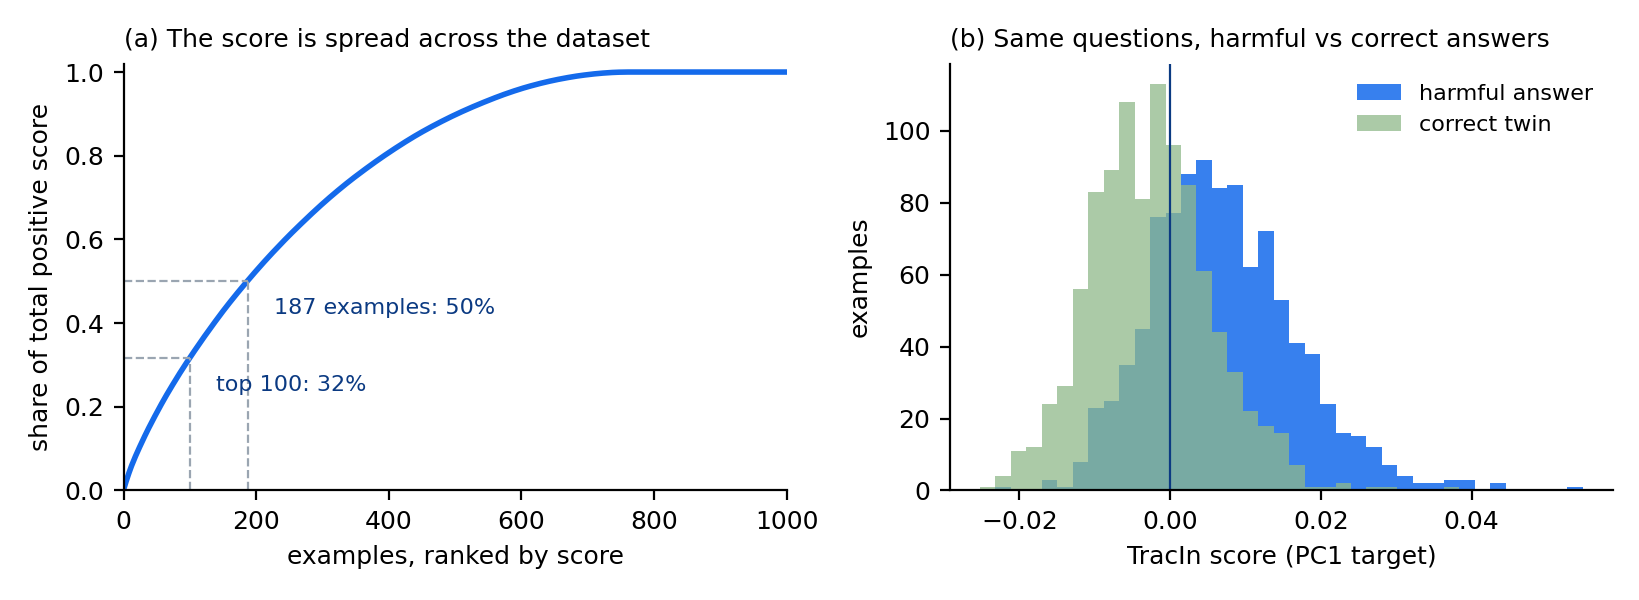
\includegraphics[width=\textwidth]{figs/orig_fig10.png}
  \caption{Scores of the reference run. (a) Share of the total positive score accounted for by the
  top-ranked examples: the top 100 account for 32\%, and 187 examples are required for half. (b)
  Score distributions of the 1,000 harmful answers and of their correct twins on the same
  questions.}
  \label{fig:e3-scores}
\end{figure}

\subsubsection{RQ2: Removal reduces the drift as predicted; the behavioural effect is not
resolved}

Table~\ref{tab:e3-retrain} reports the retrained models.
\begin{itemize}
  \item \textbf{Drift.} Removing the 100 highest-scored examples yields a final drift of 22.49,
  removing 100 random examples 24.19 on average, and removing the 100 lowest-scored examples
  26.35. The ordering follows the scores, and so does the magnitude: the summed scores of the
  removed examples predict a reduction of 2.6 points for top removal, against a realised reduction
  of 1.8 points relative to random removal. The effect amounts to roughly one noise unit per 100
  examples.
  \item \textbf{Behaviour.} Every retrained model produces fewer misaligned answers than the
  full-data model (6.7\% to 10.7\%, against 13.8\%), but removal by score is not distinguishable
  from random removal: the paired difference is $+0.9$ percentage points, with a 95\% interval
  from $-2.0$ to $+3.9$.
  \item \textbf{Utility.} GSM8K accuracy lies between 88.5\% and 91.0\% for every model.
\end{itemize}

\begin{table}[H]
  \centering
  \small
  \caption{Retraining after removal or replacement, one training seed per model. Drift is the
  final PC1 projection as a percentage of the base norm. Models trained on 900 examples end at
  optimizer step 114, the others at step 126. Misalignment rates are from the
  \texttt{gpt-5.6-sol} judge, with bootstrap 95\% intervals.}
  \label{tab:e3-retrain}
  \begin{tabular}{@{}lrrrr@{}}
    \toprule
    Training set & Examples & Final drift & Misaligned (\%) & GSM8K (\%) \\
    \midrule
    All 1,000 harmful (reference) & 1,000 & 24.26 & 13.8 [8.7, 19.6] & 88.5 \\
    Remove 100 highest-scored & 900 & 22.49 & 7.6 [4.2, 11.7] & 88.5 \\
    Remove 100 at random, draw 0 & 900 & 23.45 & 6.7 [3.1, 10.4] & 90.5 \\
    Remove 100 at random, draw 1 & 900 & 23.21 & 7.3 [3.9, 10.9] & 90.5 \\
    Remove 100 at random, draw 2 & 900 & 25.92 & 10.7 [6.3, 16.1] & 89.0 \\
    Remove 100 lowest-scored & 900 & 26.35 & 9.4 [5.1, 14.6] & 89.5 \\
    Replace 100 highest-scored by correct twins & 1,000 & 22.83 & 10.4 [5.9, 16.1] & 91.0 \\
    \bottomrule
  \end{tabular}
\end{table}

\subsubsection{Correct answers alone account for 71\% of the drift}

A run on the 1,000 correct twins, containing no harmful example, reaches a final drift of 17.31
(Figure~\ref{fig:e3-mix}a). This is 71\% of the harmful run's 24.26, so most of the drift reflects
adaptation to the medical domain rather than harmful content. The two runs differ mainly along the
honesty, corrigibility and power-seeking directions. This observation motivated the two contrast
targets, which measure drift along the direction from the all-correct run to the all-harmful run
and thereby discard the component common to both. The construction rests on an assumption that
should be stated: any other systematic difference between the two runs, such as answer length or
style, is retained in that direction as well.

\subsubsection{RQ3: The harm-specific target recovers planted examples, best at the alarm step}

Table~\ref{tab:e3-planted} reports precision at $k$ for each ranking, and
Figure~\ref{fig:e3-mix}b shows how it changes as checkpoints are added to the score.
\begin{itemize}
  \item The PC1 target exceeds chance but not the training-loss baseline.
  \item The layer-18 contrast target exceeds every baseline at the alarm step (step 40): with 100
  planted examples it places 66 of them in its top 100, against 52 for the training-loss baseline
  and 10 for chance.
  \item Scores accumulated up to step 40 outperform scores accumulated over the full run (0.66
  against 0.54 with 100 planted examples; 0.78 against 0.60 with 250). We hypothesise that the
  later checkpoints have already fit the planted examples, so that their loss gradients shrink; we
  have not tested this directly.
  \item Layer 18 was selected because projecting single-example activations onto the
  harmful-minus-benign direction separates planted from benign examples best at that layer (AUROC
  0.89 to 0.92, against 0.67 to 0.75 at layer 16, the monitor's layer). The probe was evaluated on
  the same mixtures used to report recovery, so the selection is retrospective and would need
  confirmation on an independent mixture.
\end{itemize}

\begin{figure}[H]
  \centering
  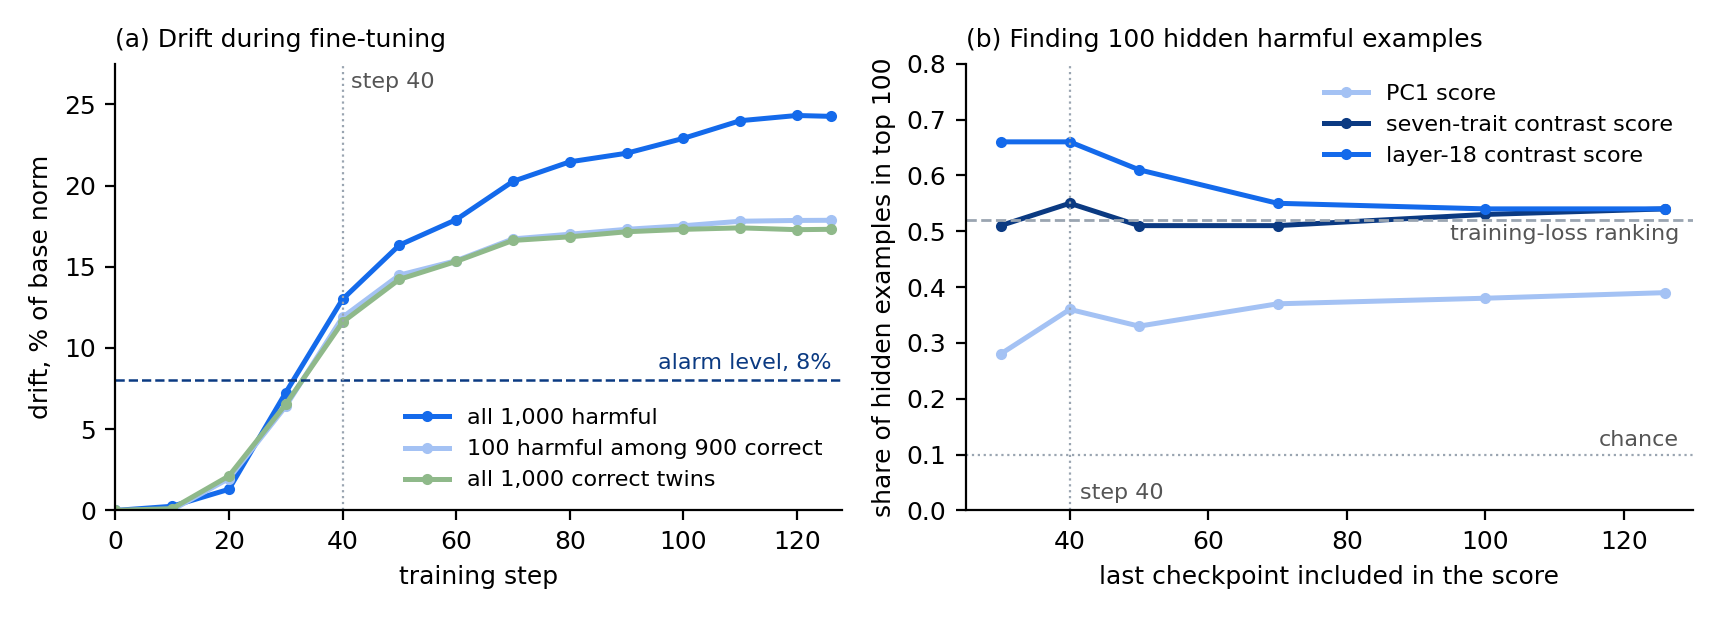
\includegraphics[width=\textwidth]{figs/orig_fig11.png}
  \caption{(a) Drift during fine-tuning for the all-harmful run, the all-correct run and the
  mixture with 100 planted harmful examples; all three exceed the 8\% reference level at
  approximately the same step. (b) Precision at $k$ for the 100-example mixture as a function of
  the last checkpoint included in the score. The layer-18 contrast target is highest when the
  alarm is raised and declines thereafter.}
  \label{fig:e3-mix}
\end{figure}

\begin{table}[H]
  \centering
  \small
  \caption{Precision at $k$, the fraction of the top-$k$ ranked examples that were planted, with
  $k$ equal to the number planted. ``Step 40'' accumulates the scores up to the step at which the
  alarm is raised; ``final'' accumulates over the full run. One permutation and one training seed
  per mixture.}
  \label{tab:e3-planted}
  \begin{tabular}{@{}llrr@{}}
    \toprule
    Planted & Ranking & Step 40 & Final \\
    \midrule
    100 of 1,000 & PC1 target & 0.36 & 0.39 \\
     & Seven-trait contrast target & 0.55 & 0.54 \\
     & Layer-18 contrast target & 0.66 & 0.54 \\
     & Training-loss baseline & \multicolumn{2}{c}{0.52} \\
     & Chance & \multicolumn{2}{c}{0.10} \\
    \midrule
    250 of 1,000 & PC1 target & 0.55 & 0.54 \\
     & Seven-trait contrast target & 0.67 & 0.63 \\
     & Layer-18 contrast target & 0.78 & 0.60 \\
     & Training-loss baseline & \multicolumn{2}{c}{0.69} \\
     & Chance & \multicolumn{2}{c}{0.25} \\
    \bottomrule
  \end{tabular}
\end{table}

\subsubsection{Threshold-based removal}

Table~\ref{tab:e3-cutoff} and Figure~\ref{fig:e3-cutoff} report the threshold variant of the
removal test. We used thresholds of $z = 2$, 1, 0.5 and 0, which flag 34, 152, 288 and 458 of the
1,000 examples. The first two bracket the fixed top-100 set, which corresponds to $z \approx 1.26$;
the last two test whether removing a larger fraction yields a proportionally larger effect.
\begin{itemize}
  \item Deleting the flagged examples yields a final drift 1.3 to 2.4 points below deleting an
  equal number of random examples at every threshold except $z = 2$, where the 34 flagged examples
  are too few to produce a measurable effect.
  \item Replacing the flagged examples by their twins yields a drift 0.1 to 1.1 points below random
  replacement at every threshold. The sign is consistent across thresholds, but each difference
  lies within noise.
  \item Smaller training sets yield fewer optimizer steps, so the absolute drift falls for both the
  flagged and the random deletion models; only the paired difference between them is
  interpretable.
\end{itemize}

\begin{table}[H]
  \centering
  \small
  \caption{Final drift after removing or replacing every example whose score exceeds the mean by
  more than $z$ standard deviations, with random controls of equal size. One training seed per
  model; the reference run reads 24.29 on the rebuilt monitor used for these runs.}
  \label{tab:e3-cutoff}
  \begin{tabular}{@{}rrrrrr@{}}
    \toprule
    $z$ & Flagged & Delete flagged & Delete random & Replace flagged & Replace random \\
    \midrule
    2 & 34 & 25.36 & 23.24 & 23.83 & 23.93 \\
    1 & 152 & 21.11 & 22.41 & 22.23 & 22.76 \\
    0.5 & 288 & 17.37 & 19.46 & 20.78 & 21.74 \\
    0 & 458 & 12.36 & 14.81 & 19.45 & 20.51 \\
    \bottomrule
  \end{tabular}
\end{table}

\begin{figure}[H]
  \centering
  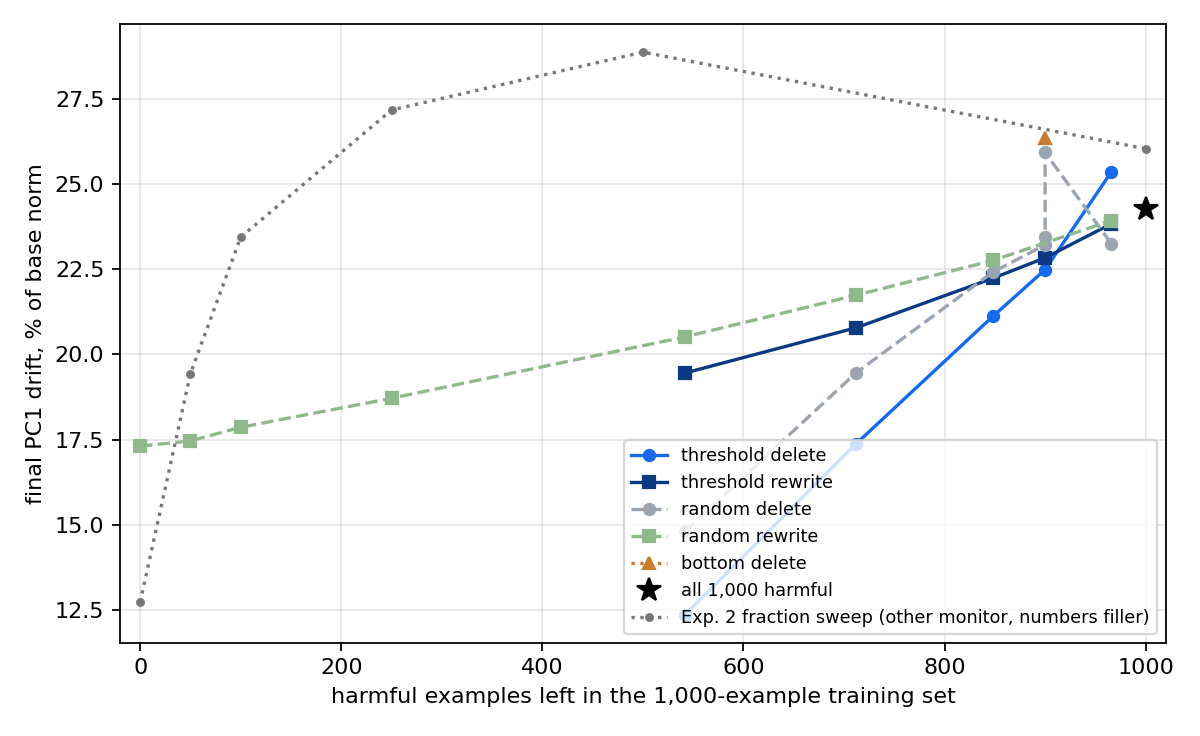
\includegraphics[width=0.85\textwidth]{figs/orig_fig12.png}
  \caption{Final drift against the number of harmful examples remaining in the 1,000-example
  training set: the threshold models of Table~\ref{tab:e3-cutoff}, the fixed-count models of
  Table~\ref{tab:e3-retrain}, and the planted mixtures. The Extension 2 sweep is shown dotted for
  its shape only; it uses a different filler dataset and a separately rebuilt monitor.}
  \label{fig:e3-cutoff}
\end{figure}

\subsection{Conclusion}

In the harmful medical run the drift is distributed across most of the 1,000 examples, and
removing or correcting the highest-scored examples reduces it by approximately the amount the
scores predict. Most of the drift on the PC1 axis, however, is produced by correct medical answers,
and a 100-example intervention did not change behaviour measurably. The harm-specific target at
layer 18 recovered two thirds of 100 planted harmful examples at the step at which the alarm is
raised, outperforming the training-loss baseline, and it performs better early in training than
late. A prospective test with a fixed layer and fixed directions, several training seeds and
additional datasets is the next step.

\end{document}
